\documentclass[8pt]{beamer}
\usetheme{default} % Very simple theme
\usecolortheme{dove} % Minimalist grayscale colors
\setbeamertemplate{navigation symbols}{} % Remove navigation bar

% Define brand-like colors
\definecolor{myblue}{RGB}{0, 102, 204}    % Blue for standard blocks
\definecolor{mygreen}{RGB}{0, 153, 0}     % Green for example blocks
\definecolor{myred}{RGB}{204, 0, 0}       % Red for alert blocks
\definecolor{myorange}{RGB}{255, 128, 0} % For \emph

% Accent color for titles, bullets, etc.
\setbeamercolor{structure}{fg=myblue}

% Block colors
\setbeamercolor{block title}{bg=myblue, fg=white}
\setbeamercolor{block body}{bg=blue!5, fg=black}

\setbeamercolor{exampleblock title}{bg=mygreen, fg=white}
\setbeamercolor{exampleblock body}{bg=green!5, fg=black}

\setbeamercolor{alertblock title}{bg=myred, fg=white}
\setbeamercolor{alertblock body}{bg=red!5, fg=black}
\setbeamercolor{alerted text}{fg=myred}

% Optional: color for \example text
\setbeamercolor{example text}{fg=mygreen}

% Custom emph (orange text instead of italic)
\let\oldemph\emph
\renewcommand{\emph}[1]{\textcolor{myorange}{#1}}


\usepackage{graphicx} % Package for images
\usepackage{amsmath} % Package for images
\graphicspath{{figs/}} % Path to your figures directory
\usepackage{array}  % For better column spacing
\usepackage{caption} % Required for \captionof

% Title Information
\title{STOCHASTIC METHODS IN WATER RESOURCES}
\vspace{25pt}
\subtitle{Unit 2: Hydrological statistics and extremes \\ Lecture 8: Hydrological design, Makov chains and regional frequency analysis}
\author{Luis Alejandro Morales, Ph.D.}
\institute{Universidad Nacional de Colombia \\ Department of Civil and Agriculture Engineering} %// }
%\date{\today}

\begin{document}

% Title Slide
\begin{frame}
    \titlepage
\end{frame}

%-------
% From Diaz-granados
\section{Hydrologic design}
\subsection{Generalities}
\begin{frame}{Hydrologic design}
   \begin{block}{Generalities}
   \end{block}
   \begin{itemize}
       \item \emph{Planning and management} of water resources can be classified according to their 1) \alert{use} (e.g. Hydroelectricity, water supply, recreation, etc) and their 2) \alert{control} (e.g. drainage, flood, contamination, sedimentation, etc.). 
       \item The \alert{hydrologic design} for \emph{control} is relate to extreme events of short duration (e.g. a flood). The optimal design is a balance between the cost and safety of the designed structure. 
       \item Regarding that water is finite on earth,  extreme hydrological events have \emph{limit values} that are difficult to know and thus are quite uncertain. For \emph{precipitation} data, the superior limit is defined by the \emph{probable maximum precipitation (PMP)} and for \emph{streamflow} data it is defined by the \emph{probable maximum flood (PMF)}. This limits are used for instance in the design of excess spillways in reservoir.
       \item The estimation of the limits is deterministic so that the limits do not obey to a \emph{return period}. An structure designed based on those limits  might support all possible of hazards. 

       
   \end{itemize}
\end{frame}

\begin{frame}{Hydrologic design}
   \begin{block}{Generalities}
   \end{block}
   \begin{itemize}
      \item When the limits are not considered, the \emph{hydrologic design} of the structure is based on frequency analsis, where the magnitude of the hydrological variable of interest is estimated for certain \emph{design return period ($T_D$)}. For instance,   for $T_D =100$ yr the corresponding value of the design hydrological variable is expected to be exceeded in average once every 100 yr, or that the probability of the occurrence of that event in a given year is $1/T_D = 0.01$, which is quite low. 
       \item Note that when a structure is design for a $T_D$, there is a \emph{residual hazard} because  there is a probability that a larger event occur during the \emph{structure's design life}.

       \item To estimate the magnitudes of the design hydrological variables is needed to obtain the \emph{frequency curves}; a methodology that has been explained before here. Note that the \emph{frequency curves} are obtained assuming that the data sample (e.g. annual time series of extreme rainfall) comes from a \emph{stationary process}.  
   \end{itemize}
\end{frame}

\begin{frame}{Hydrologic design}
   \begin{block}{Definition of design return period ($T_D$)}
   \end{block}
   \begin{itemize}
       \item A design of a structure can be based on the \alert{design return period ($T_D$)}. Their definition is based on \emph{design manuals} or \emph{design codes} (e.g. manual de  diseño del INVIAS o de la EAAB). Also, the $T_D$ can be established after \emph{risk analysis in hydrology} or from \emph{economical analysis}, these two allow estimate an optimal $T_D$. 
       \item The magnitude to the hydrological design variable is obtained from the \emph{frequency curve} using $T_D$. However, it is important to follow the recommendation given by design manuals and codes regarding the type of \emph{probability distributions} to be implemented and the methods to estimate their parameters. For instance, in USA agencies is recommended to use the \emph{Log Pearson type III} for the analysis of maximum streamflows. 
   \end{itemize}

   \alert{How to determine $T_D$?}\\

              \begin{itemize}
                  \item According to the type of structure, and based on previous engineering experience and the recommendations given by design manuals and codes, a value or a range of values for $T_D$ is given. For instance, for the design of highway drainage systems it is recommended $5 yrs \leq T_D \leq 100 yrs$, where the value depends on the traffic volume. Similarly, while a $2 yrs \leq T_D \leq 25 yrs$ is recommended for pluvial sewage systems in small cities, a $25  yrs \leq T_D \leq 50 yrs$ is recommended for large cities. 
                  \item Based on government policies, the level of hazard can dictate the range of $T_D$. So for instance, in coastal cities, the risk of floods can be higher so for the design of  coastal levees,  $T_D$ can be up to 10000 yrs. 
                      

              \end{itemize}
\end{frame}

\begin{frame}{Hydrologic design}
   \begin{block}{Definition of design return period ($T_D$)}
   \end{block}
    \alert{How to determine $T_D$?}\\
   
    \begin{itemize}
        \item In Colombia, the \alert{RAS 2000} technical regulations, stablish that a $2  yrs \leq T_D \leq 50 yrs$ for the design of combine or pluvial sewage systems. The ultimate value of $T_D$ will depend on the use,  slope, area, etc of the system. The \alert{INVIAS} stablish the following $T_D$ for the design of highways structures:
                      \begin{itemize}
                          \item \emph{Gutters}: $T_D = 5 yrs$
                          \item \emph{Culvert $\phi = 0.9$ m}: $T_D = 10 yrs$
                          \item \emph{Culvert $\phi > 0.9$ m}: $T_D = 20 yrs$
                          \item \emph{Bridge $10 m \leq \text{ span } \leq 50 m$}: $T_D = 50 yrs$
                          \item \emph{Bridge $\text{ span } > 50 m$}: $T_D = 100 yrs$
    \end{itemize}
    \end{itemize}
 
    \alert{Selection of $T_D$ based on hydrological risk}\\
         To estimate $T_D$ is assumed a value for the \alert{hydrological risk ($R_h$)}. Recall that $R_h$ is defined as the probability that the hydraulic capacity of the structure is exceeded by a hydrological hazard once during the expected life of the structure ($n$ yrs). Accordingly
            \[
                T_D = \frac{1}{1- (1-R_h)^{1/n}}
            \]

\end{frame}

\begin{frame}{Hydrologic design}
   \begin{block}{Definition of design return period ($T_D$)}
   \end{block}
   \vspace{-7pt}
    \alert{Selection of $T_D$ based on hydrological risk}\\
 \begin{minipage}{0.48\textwidth}
     \begin{itemize}
         \item The table shows the values of $T_D$ for different values of $R_h$ and $n$. Note that the lesser $R_h$ the higther $T_D$. In contrast, the larger $n$ the highter $T_D$. Remember that when $T_D = n$, $R_h \approx 0.63$, which is quite high. 
         \item For instance, in the design of a cofferdam and a diversion tunnel, it is common to adopt a streamflow design for a $T_D = 50$yrs, which correspond to $R_h = 0.096$ or 9.6\% for $n = 5$yrs. This contrast, $T_D$ for a \emph{design seismic earthquake}, according to the design codes in Colombia, is equal to 475 yrs, which correspond to $R_h = 0.1$ and $n=50$yrs. 
     \end{itemize}
\end{minipage}
\hfill
\begin{minipage}{0.48\textwidth}
    \centering
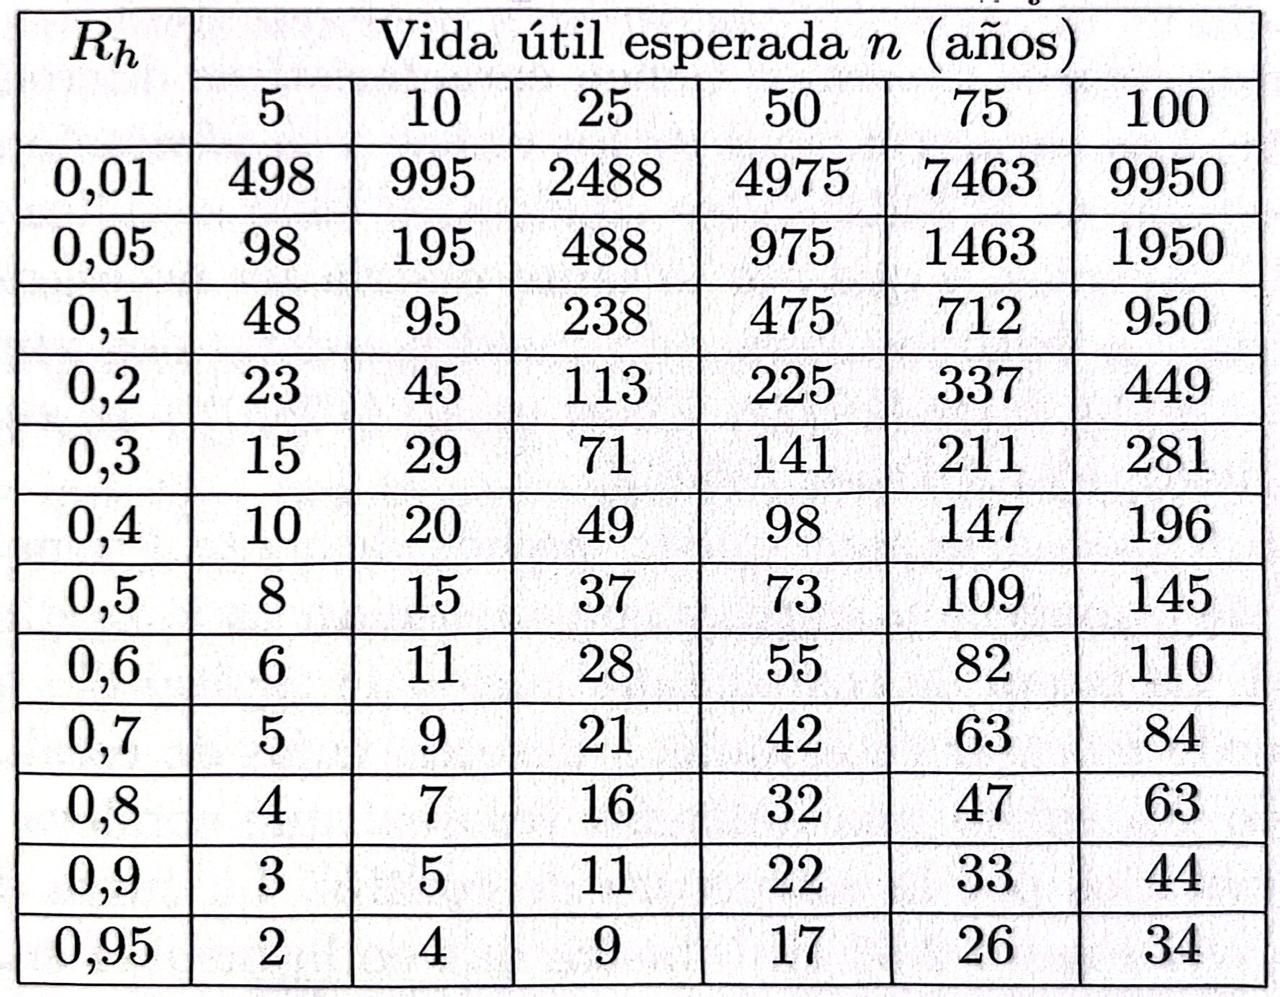
\includegraphics[width=1\linewidth]{taM288.jpeg}  % from Diaz-Gra
\end{minipage}
Conversely, 
\vspace{-5pt}
\[
    R_h = 1-\left(1-\frac{1}{T_D} \right)^n
\]
Note that when $T_D$ is low, $R_h$ is total (absolute certainty of the occurrence of the event during $n$). For instance for the case of a pluvial sewage system, when $T_D = 2$ yrs and $n=25$yrs, $R_h \approx 1$. This means that with total certain the sewage system will experiment at least once an event that exceed its hydraulic capacity.There are other uncertainty associated to the structural design, construction, operation, etc.  
\end{frame}

\begin{frame}{Hydrologic design}
   \begin{block}{Definition of design return period ($T_D$)}
   \end{block}
    \alert{Selection of $T_D$ based on economical analysis}\\
\end{frame}

\end{document}

